Un arbre binaire de recherche présente-t-il un avantage par rapport à une table de hachage pour réaliser un \textit{Map} ? Pourquoi ? Et par rapport à une \textit{Skip List} ? \\
La forme d’un arbre binaire de recherche dépend-elle de l’ordre d’insertion des clés ? La forme d’un arbre binaire de recherche dépend-elle de l’ordre de suppression des clés ? Quelle est la complexité temporelle de l’insertion de $\textit{n}$ clés identiques dans un arbre binaire de recherche initialement vide ? Quelle est la propriété particulière des arbres binaires de recherche qui justifie l’intérêt d’autres structures de données comme les Arbres AVL ou les Arbres (2,4) ? (\textbf{Sundeep}) \\
\bigskip

Si on utilise un arbre binaire de recherche, l'avantage principal est lié à l'efficacité des méthodes qui ne seront plus en complexité temporelle $O(n$) mais bien en $O(log (n))$ dans le meilleur des cas et ce, surtout si l'arbre est équilibré. Au contraire, dans le pire des cas, la complexité temporelle sera en $O(n)$ vu que l'arbre n'est pas du tout équilibré et donc, la hauteur est de $n$. \\

Face à une \textit{Skip List}, cet avantage n'en est plus un vu que la complexité temporelle dans ces deux cas est identique. \\ 

La forme d'un arbre binaire de recherche dépend effectivement de l'ordre dans lequel on ajoutera ou supprimera des clés. Si l'on ajoute les clés dans l'ordre croissant (ou décroissant), l'arbre ne sera dans plus du tout équilibré et aura une hauteur de $n$. La meilleure chose à faire serait d'ajouter les différentes clés en prenant les clés centrales. \\
Lors de la suppressions de clés, les vides sont compensés du fait qu'on va aller chercher la clé la plus à gauche du fils de droite pour remplir le vide créé. Ces suppressions peuvent donc bel et bien influencer la forme de l'arbre. \\

La complexité temporelle de l'insertion de $\textit{n}$ clés identiques dans un arbre binaire de recherche initialement vide sera de $O(n^2)$. A chaque ajout $n$, on devra parcourir l'entièreté de l'arbre. Le fait de devoir donc multiplier $n$ par $n$ explique bien le pourquoi du $n^2$. \\ 

La particularité des arbres binaire est que la complexité des méthode de bases varie entre O(n) et O(log n). On cherchera donc a maximiser l'apparition des situation dans lesquels la complexité se limitent à O(log n). \\
 
Pour ce qui concerne l'intérêt d'autres structures de données comme les Arbres AVL, il s'agit tout simplement d'essayer d'avoir une complexité temporelle de base qui varie entre $O(n)$ et $O(log (n))$ pour les principales opérations. Pour ce faire, nous allons maximiser l'obtention de situations telles que la complexité se limite à $O(log (n))$ et la seule correction à effectuer consiste à ajouter une règle à la définition de l'arbre binaire de recherche pour maintenir une hauteur en logarithme pour l'arbre. La règle en question est la \textbf{propriété d'équilibre de l'hauteur}, celle-ci caractérise la structure d'un arbre binaire de recherche \textit{T} en termes des hauteurs de ses noeuds internes. Autrement dit, pour chaque noeud interne $\textit{v}$ de \textit{T}, les hauteurs des enfants de $\textit{v}$ diffèrents de 1 au maximum. Tout arbre binaire de recherche \textit{T} qui satisfait cette dernière propriété est appelé un \textbf{Arbre AVL\footnote{Ce nom provient de ses inventeurs, à savoir: Adel'son-Vel'skii et Landis}}. Une conséquence directe de cette propriété est qu'un sous-arbre d'un arbre AVL est d'office un arbre AVL. Une autre propriété est que la hauteur d'un arbre AVL pour stocker $\textit{n}$ entrées est $\textit{O}(log (\textit{n}))$.

\begin{figure} [!h]
\center
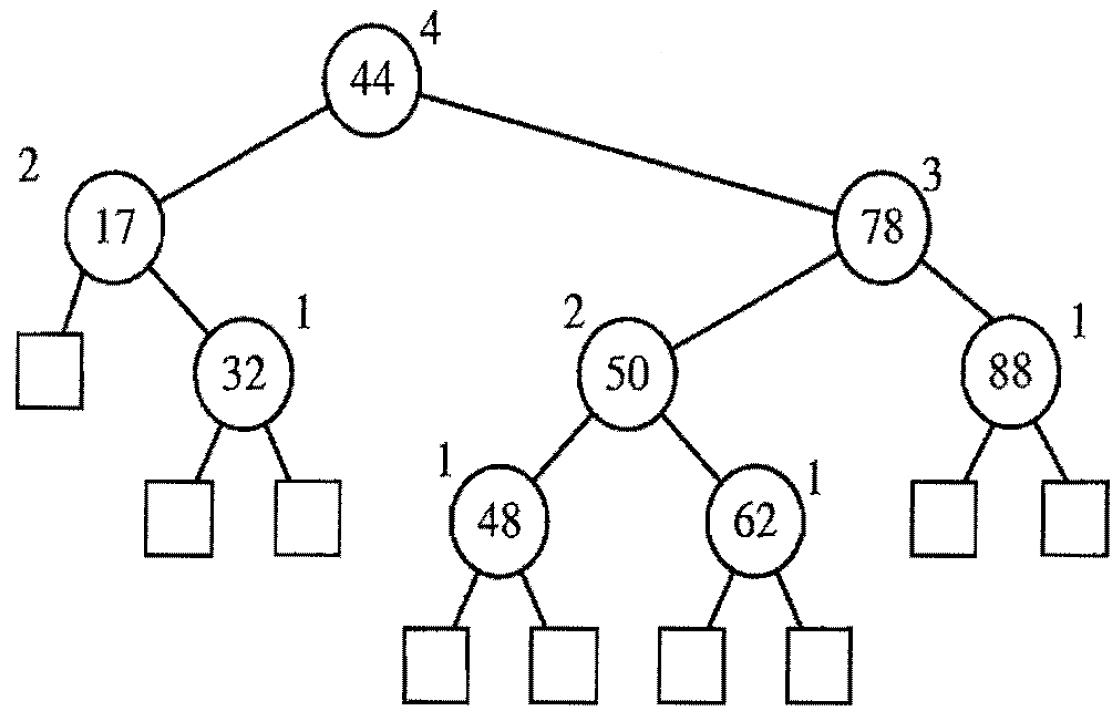
\includegraphics[scale=0.37]{AVL.png}
\caption{Exemple d'arbre AVL. Les clés des entrées sont mises à l'intérieur des noeuds et les hauteurs des noeuds sont indiquées à côté de ces derniers.}
\end{figure}